\documentclass[11pt]{article}
\usepackage{lmodern}
\usepackage{amssymb,amsmath}
\usepackage{ifxetex,ifluatex}
\usepackage{fixltx2e} % provides \textsubscript
\ifnum 0\ifxetex 1\fi\ifluatex 1\fi=0 % if pdftex
  \usepackage[T1]{fontenc}
  \usepackage[utf8]{inputenc}
\else % if luatex or xelatex
  \ifxetex
    \usepackage{mathspec}
    \usepackage{xltxtra,xunicode}
  \else
    \usepackage{fontspec}
  \fi
  \defaultfontfeatures{Mapping=tex-text,Scale=MatchLowercase}
  \newcommand{\euro}{€}
\fi
% use upquote if available, for straight quotes in verbatim environments
\IfFileExists{upquote.sty}{\usepackage{upquote}}{}
% use microtype if available
\IfFileExists{microtype.sty}{%
\usepackage{microtype}
\UseMicrotypeSet[protrusion]{basicmath} % disable protrusion for tt fonts
}{}
\ifxetex
  \usepackage[setpagesize=false, % page size defined by xetex
              unicode=false, % unicode breaks when used with xetex
              xetex]{hyperref}
\else
  \usepackage[unicode=true]{hyperref}
\fi
\usepackage[usenames,dvipsnames]{color}
\hypersetup{breaklinks=true,
            bookmarks=true,
            pdfauthor={},
            pdftitle={},
            colorlinks=true,
            citecolor=blue,
            urlcolor=blue,
            linkcolor=magenta,
            pdfborder={0 0 0}}
\urlstyle{same}  % don't use monospace font for urls
\usepackage{longtable,booktabs}
\usepackage{graphicx,grffile}
\makeatletter
\def\maxwidth{\ifdim\Gin@nat@width>\linewidth\linewidth\else\Gin@nat@width\fi}
\def\maxheight{\ifdim\Gin@nat@height>\textheight\textheight\else\Gin@nat@height\fi}
\makeatother
% Scale images if necessary, so that they will not overflow the page
% margins by default, and it is still possible to overwrite the defaults
% using explicit options in \includegraphics[width, height, ...]{}
\setkeys{Gin}{width=\maxwidth,height=\maxheight,keepaspectratio}
\setlength{\parindent}{0pt}
\setlength{\parskip}{6pt plus 2pt minus 1pt}
\setlength{\emergencystretch}{3em}  % prevent overfull lines
\providecommand{\tightlist}{%
  \setlength{\itemsep}{0pt}\setlength{\parskip}{0pt}}
\setcounter{secnumdepth}{0}

\date{}

% Redefines (sub)paragraphs to behave more like sections
\ifx\paragraph\undefined\else
\let\oldparagraph\paragraph
\renewcommand{\paragraph}[1]{\oldparagraph{#1}\mbox{}}
\fi
\ifx\subparagraph\undefined\else
\let\oldsubparagraph\subparagraph
\renewcommand{\subparagraph}[1]{\oldsubparagraph{#1}\mbox{}}
\fi

\setlength{\oddsidemargin}{-0.1in}
\setlength{\topmargin}{-0.52truein} 
\setlength{\textheight}{9.15in} 
\setlength{\textwidth}{6.7in}

\usepackage[T1]{fontenc}
\usepackage{fourier}
\usepackage[sc]{mathpazo}
\linespread{1.05}         % Palatino needs more leading (space between lines)


\usepackage{wrapfig}
\usepackage[square,numbers,sort&compress]{natbib}
\renewcommand{\cite}{\citep}
%\usepackage[psamsfonts]{amssymb}
%\usepackage{palatino}
%\usepackage{mathpazo}

%\usepackage{plasmadefs}

\hyphenation{wave-packet wave-packets}

\title{}

\begin{document}

\section{Facilities and Infrastructure}

\subsection{Large Plasma Device {LAPD}}
The LAPD  is housed in a vault with an area of 3300 sqft.\ (30 x 110) and 18 foot ceiling; it has a 2.5 ton overhead crane.  The magnet power supplies and heat exchangers are adjacent in a 900 sqft.\ space.  The machine vault was originally designed to accommodate a free electron laser so that the room is radiation hardened with the walls and ceiling made from five-foot-thick, triple-density concrete with two inch re-bar.  Adjacent to the machine vault are two 600 sqft.\ (20 x 30) rooms.  One serves as the control and data acquisition room while the other houses the LIF and pulsed lasers.
	The LAPD plasmas are generated by electrons emitted from a heated, barium oxide-coated cathode and subsequently accelerated by a semi-transparent grid anode located near the cathode.  The ionizing electrons ($\sim$ 50 eV) strike an inert, neutral gas (e.g., Helium or Argon) and generate highly ionized (up to fully ionized) plasmas. Highly reproducible, quiescent plasmas are formed, having typical discharge duration of 1-10 ms at a 1 Hz repetition rate.  After the discharge pulse is terminated, the electron temperature falls rapidly but the plasma density remains confined for relatively long times, thus permitting additional access to experimentation in afterglow conditions for intervals exceeding 50 ms. The heater assembly for the cathode can withstand the $J\times B$ forces encountered at the largest magnetic field values (2.5 kG).
	The LAPD plasma column has a maximum length of 18 meters and 75-centimeter diameter.  Plasmas of varying length can be explored by segmenting the device (i.e., inserting a terminating copper end plate at various axial locations).  The confining magnetic field can achieve a steady-state value of up to 2.5  kG.  Ordinarily the magnetic field is uniform, but it be can be configured to create multiple or single mirror geometries, magnetic cusps, axial field gradients and other configurations of scientific interest.  The cathode is driven by a 4-Farad capacitor bank that can supply a total discharge current of 32 kA.  The electron source is switched by banks of 2.5 kA, 1.5 kV transistors. 
	
	The length of the plasma column and the radial density profiles can be tailored to study various physical processes that depend on transverse or axial gradients in density and temperature.  Plasmas are routinely available with densities up to $4\times 10^{12}$ cm$^{-3}$ and electron temperatures in the 1-15 eV range. Presently the ion temperature is fixed by the discharge dynamics at approximately 1 eV.  There are plans to add RF heating to vary the ion temperature.
 	The LAPD has unprecedented access with eight, 12 cm diameter access ports between each magnet set (424 in total) including eight, unique "octo-ports".  The octo-ports encircle the entire plasma column and have eight, 10 x 40 cm, rectangular openings, which allow for a nearly unimpeded 360$^{\circ}$ view.  These ports can be used for visible and microwave tomography, laser fluorescence, or the insertion of various large antennas, smaller plasma sources, or plasma-terminating end plates.  A composite photograph of the device is shown in Figure \ref{fig:LAPD}(a), with a corresponding schematic representation in Figure \ref{fig:LAPD}(b).
	\begin{figure}[htbp] %  figure placement: here, top, bottom, or page
	   \centering
	   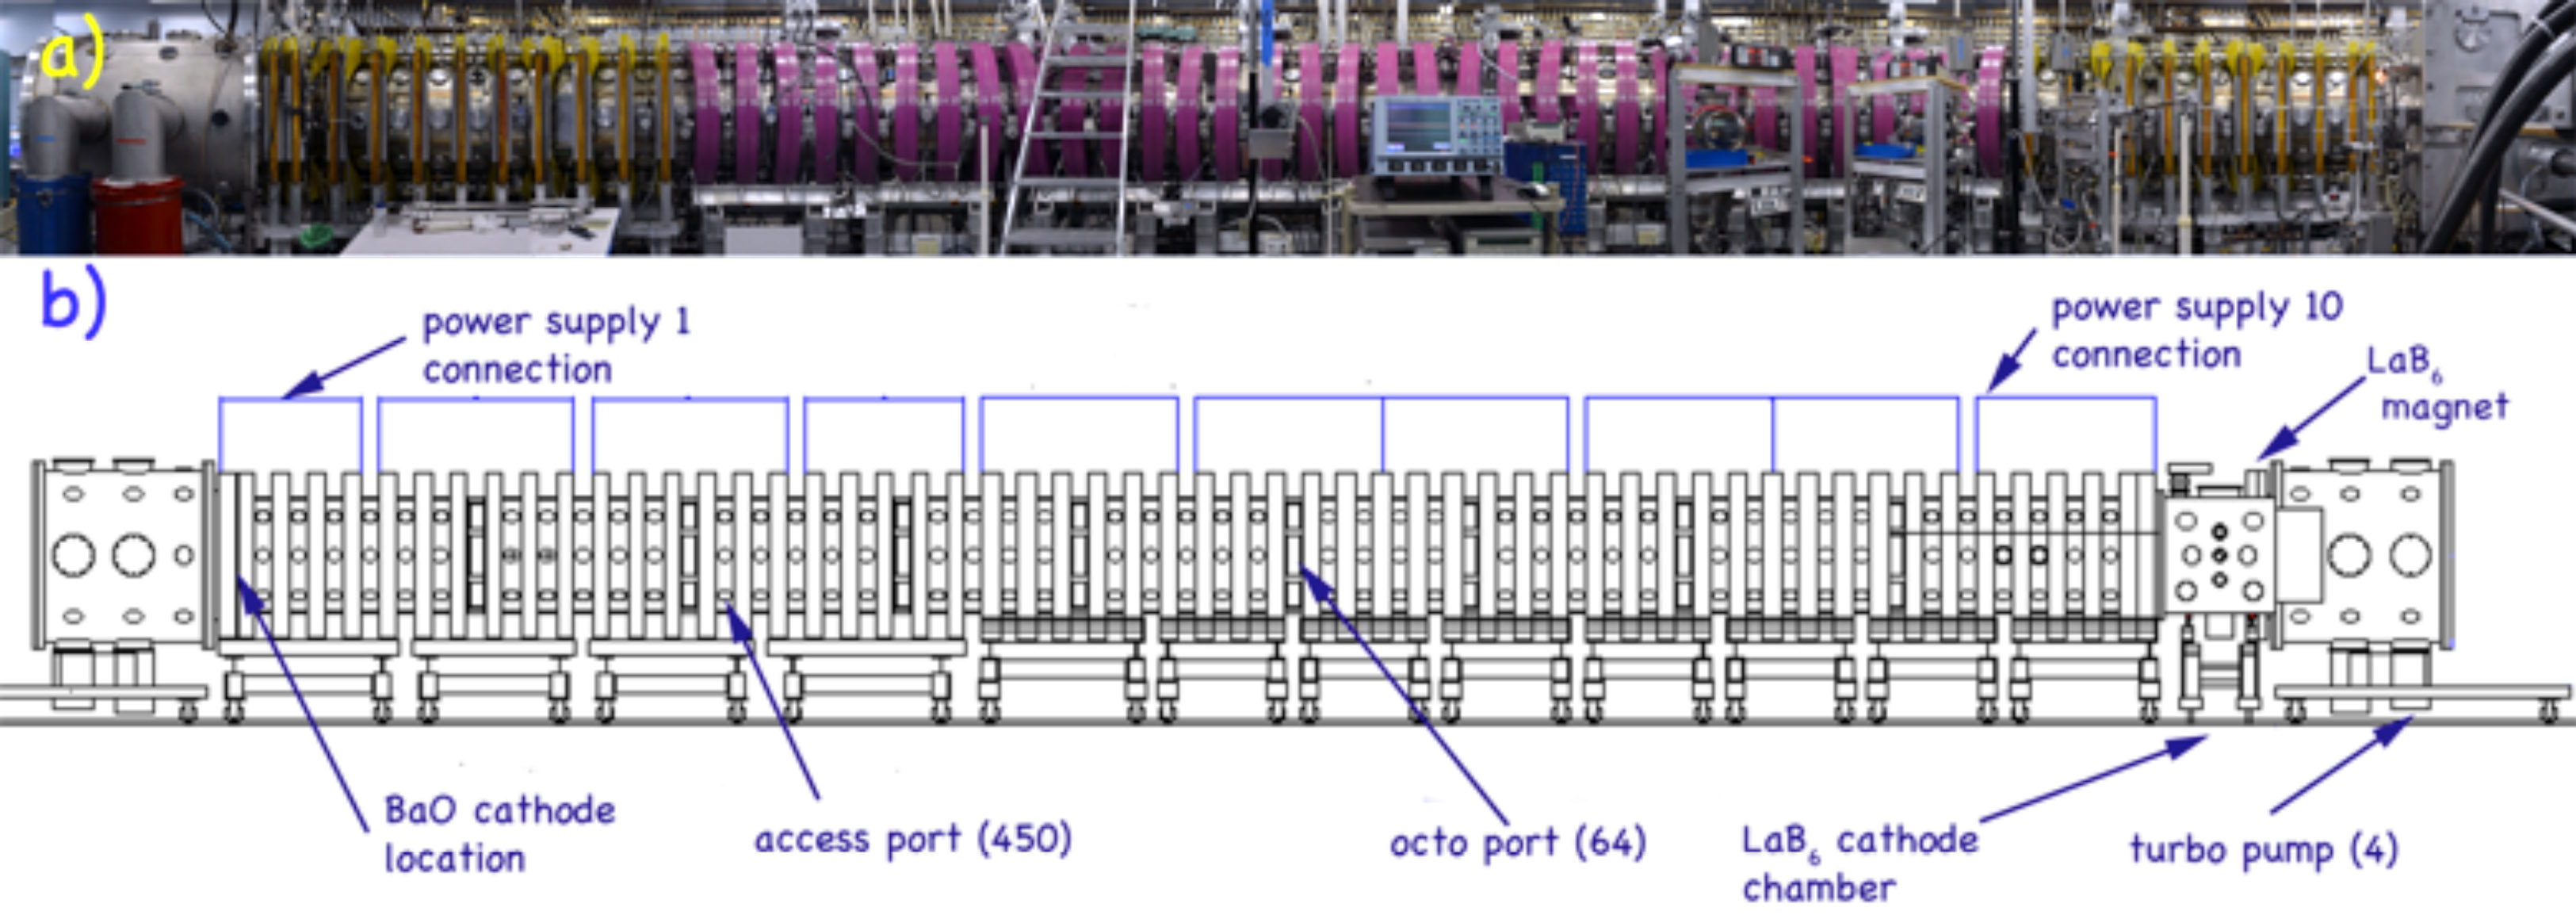
\includegraphics[width=6.5in]{LAPD.jpg} 
	   \caption{(a) Composite photograph of the LAPD.  Shown on the left is a pump-out chamber, which contains the BaO cathode and two of the four 2200 L/s, turbo-molecular pumps. The magnets and ports fill most of the scene and the chamber containing the Lanthanum Hexaboride second cathode is on the right.  The entire machine is 24.4 meters end-to-end. (b) Machine drawing showing the two types of ports as well as the connections to the power supplies. An additional magnet is used to provide a magnetic field at the second LaB$_{6}$ cathode. }
	   \label{fig:LAPD}
	\end{figure}
	
	The LAPD magnetic coil system consists of 92 individual pancake magnets placed along the machine length. The magnets are controlled by ten separate power supplies, specifically designed for this system.  The power supplies can be controlled manually or by computer, and allow operation of up to 2.5 kG uniform axial magnetic field with 0.1\% current ripple.  The magnet power supplies (4 supplies: 9.6 kA, 40 V; 6 supplies : 3600 A, 84 V) are fed by a 4.0 MW substation acquired for this project.  An additional MW of power is available in the laboratory for general use.  The building is unique in its electrical capabilities; it is designed to accommodate large experiments that require high power levels.  Presently there is 15 MW available in the building switchyard, and this can be doubled if necessary.
	
	In the summer of 2004, UCLA paid for a significant upgrade of the LAPD cooling system.  Fifty degree (F) chilled water was routed into the laboratory from a nearby chilling plant.  UCLA also paid for an air conditioning system in the laboratory capable of cooling a 100 kW load. 

Three pump-down stations comprising a cryopump and mechanical pump, ionization gauges, mass analyzers, and vacuum fittings enable users to move instrumentation in and out of the device.  The main vacuum system relies on four turbo pumps with a combined pumping speed of 9000 L/s.  Two Stanford residual gas analyzers with computer interfaces monitor the vacuum and gas evolution during cathode conditioning.   A gas mixing system using mass flow controllers allows for the mixing of up to six neutral gases in variable, yet precise ratios.

		It is possible to connect several (up to four), computer-controlled, probe drive systems at once through any one of 50 adjacent ports on either side along the machine axis.  If the need arises, simultaneously activated probes can acquire data at several spatial locations in the plasma volume.  Probes may be introduced during machine operation using vacuum interlocks and the portable cryo-based pumpdown stations. 
		
		
		In the summer of 2013, a major upgrade to the LAPD was installed: a second, Lanthanum Hexaboride (LaB$_{6}$) cathode (20cm x 20cm)  source was added to the LAPD on the end opposite to the barium-oxide source. A rendering of the cathode and one-meter extension chamber is shown in Figure \ref{fig:lab6cartoon}. The advantage of LaB$_{6}$ is that its emission is ten times that of barium oxide (the cathode coating material presently in use in the LAPD), it is not easily spoiled by O$_{2}$ impurities, and may be driven to higher discharge voltage (presently tested to 350V) because it is not easily destroyed by ion bombardment.  The disadvantage is that it must be heated to 1450-1550 C before it emits rather than 850-900 C for BaO.  Since the radiant heat is proportional to the fourth power of the temperature, a cathode using LaB$_{6}$ produces 5 times the heat of one using BaO .  This large heat load is dissipated by aggressive cooling of the chamber wall and support structures.   This new source successfully generates a 20cm diameter (1/3 the background column diameter) dense ($\sim 3\times 10^{13}$cm$^{-3}$) hot ($T_{e}=15$eV, $T_{i}=2-4$eV) plasma column embedded in a pre-existing plasma.  The two cathode pulsers and the timing circuitry are independent so that the second plasma can be pulsed-on, during or after, the main discharge. Since its initial installation, approximately 50\% of facility users have requested experiments which utilize the new cathode.

\begin{figure}[htbp] %  figure placement: here, top, bottom, or page
   \centering
   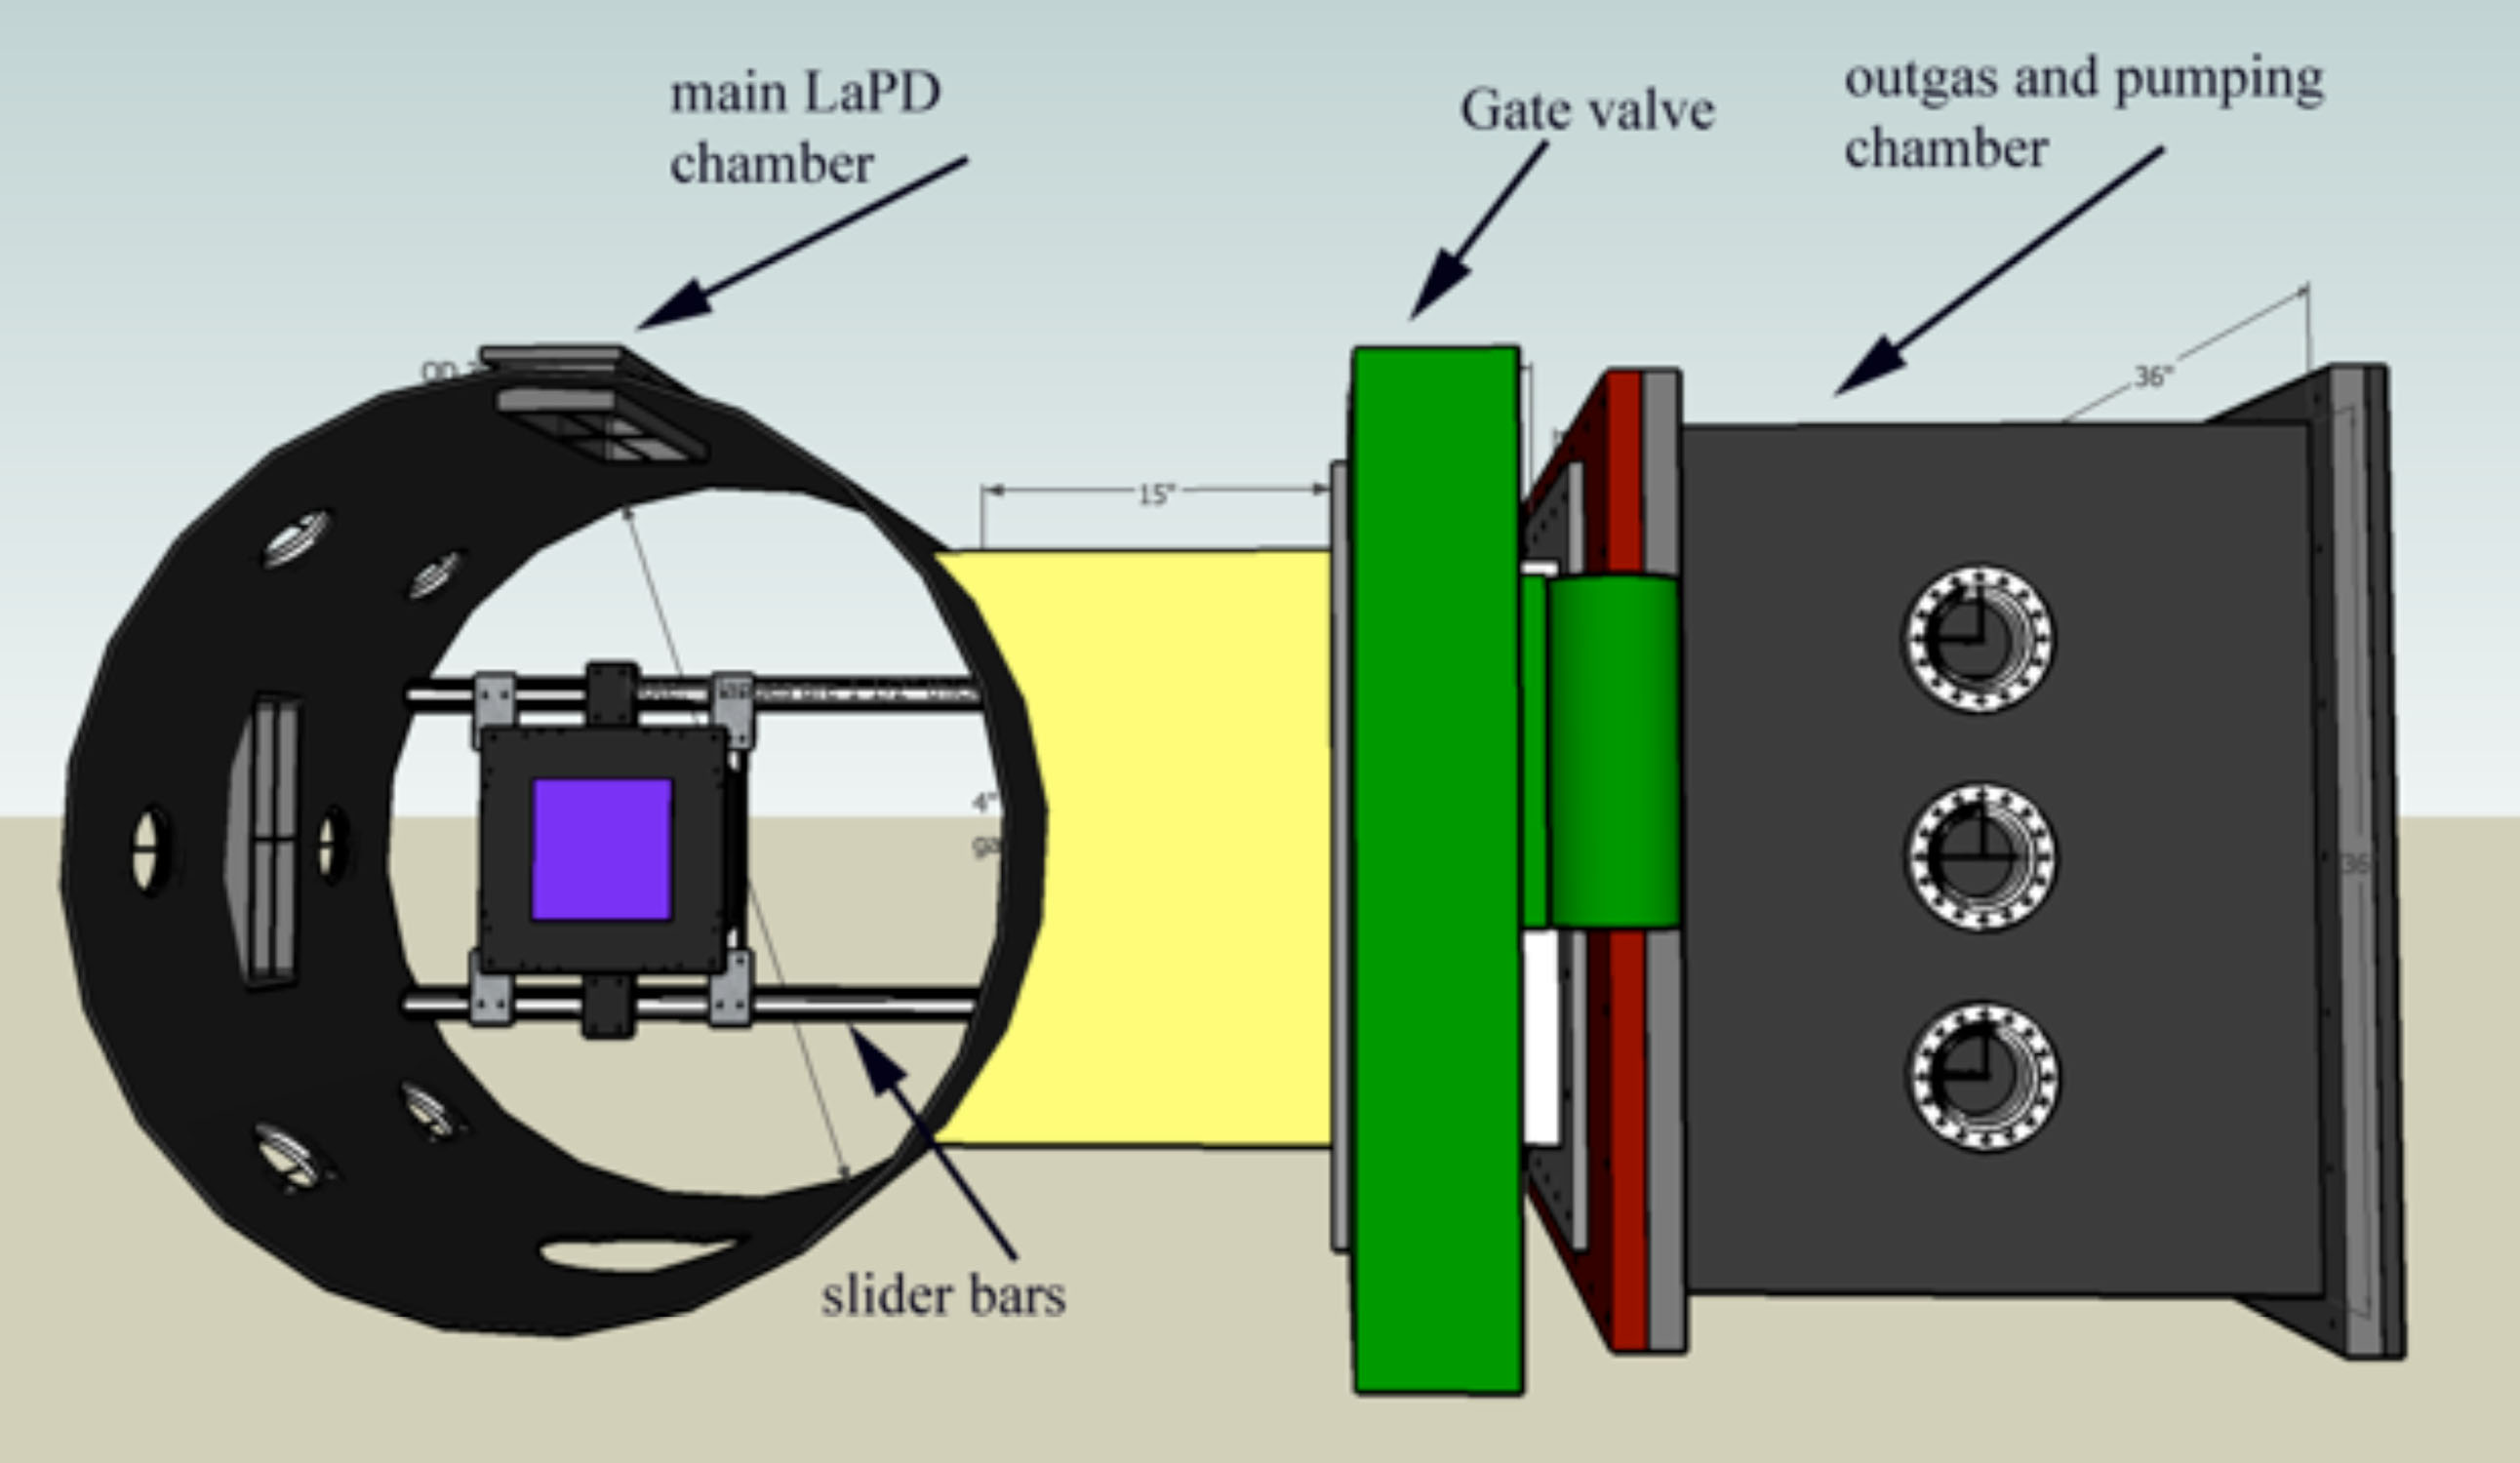
\includegraphics[width=6in]{lab6cartoon.jpg} 
   \caption{Drawing of the new chamber and LaB$_{6}$ cathode system installed on the LAPD.  The LaB$_{6}$ cathode, shown as a purple square, is on slider bars that allow it to be fully retracted from the machine.  The cathode can be moved into the out-gassing chamber on the right, and can be separated from the main vacuum chamber using a large gate valve (green).  The chamber has a dedicated turbo pump (donated from industry) and all the power and water-cooling lines necessary for the cathode.  A water-cooled copper shroud was installed in the LAPD and in the out-gassing chamber to cool them.}
   \label{fig:lab6cartoon}
\end{figure}
		
		


\subsection{The Enormous Toroidal Plasma Device (ETPD)}
The ETPD device is housed on the main floor of the STRB building.  The device was originally constructed as a tokamak and if run in that mode, it would still be the physically-largest tokamak in the world.  The vacuum system interior dimensions are 2 m wide and 5 m high.  The chamber is made from 1inch-thick stainless steel.  The 32 toroidal magnets are made of Al slabs separated by glass insulators.  Magnets plus chamber weigh in at 300 tons. The device is shown in Fig.\ ref{fig:etpd}.   The long-term vision of BaPSF is to convert this chamber into a 24/7 operating basic plasma device with diagnostic capabilities equal to the LAPD. To attain that level of performance a separate infrastructure grant will be pursued in the future. 

Figure \ref{fig:etpd2} is a photograph of the ETPD plasma together with profiles, across the plasma column, of measured plasma parameters.  The ETPD and its immediate diagnostics occupy 5760 sqft.\ of high-bay space.  This area has a 25 foot ceiling and a 10 ton crane.  There is an additional 2880 sqft.\ of low bay space for power supplies to service the ETPD.  There is 1.3 MW available raw power fed by 12 kV lines and an additional 3 MW of 480/220 power in ?rails? lining the walls surrounding ETPD to which circuit breakers may be attached.  The STRB also has 2048 sqft.\ of machine shop space to service the building.  The machines available include end mills and lathes (both manual and computer-controlled); band-saws; several welders; and cut-off saws.  Presently the plasma source has a 20 cm diameter LaB$_{6}$ cathode and plans are underway to upgrade this to a 60 cm source.
\begin{figure}[h] %  figure placement: here, top, bottom, or page
   \centering
   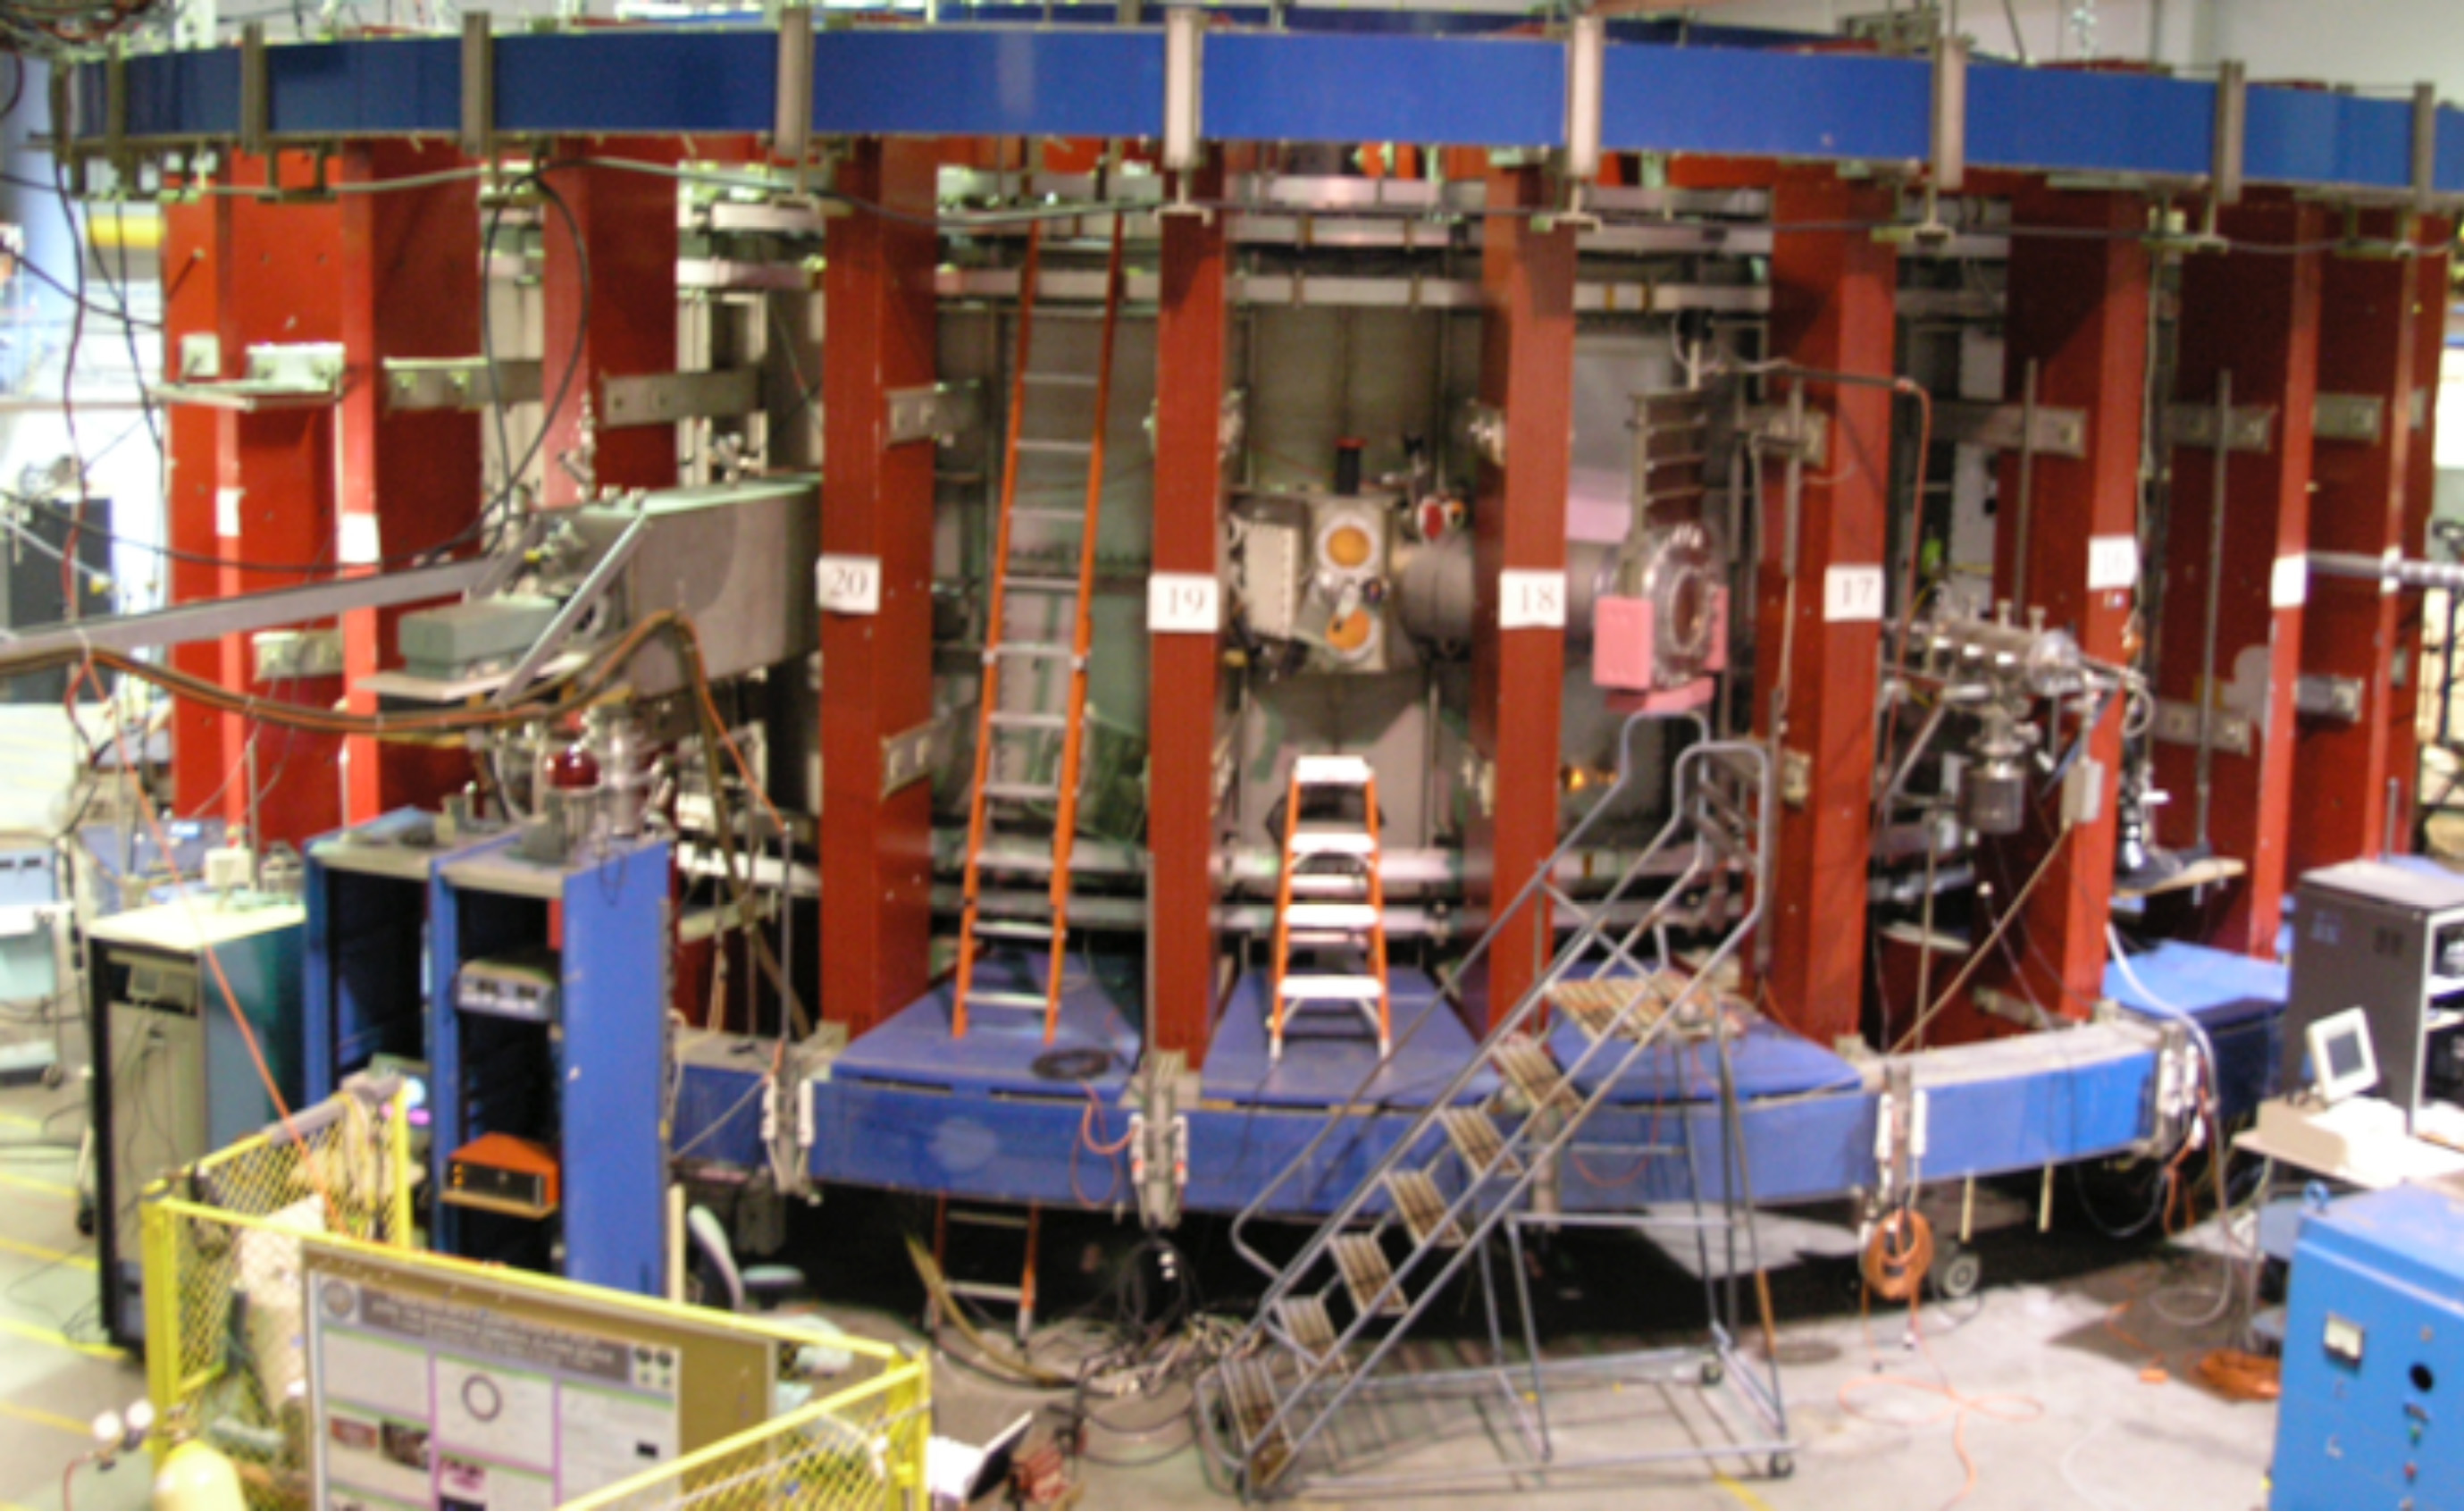
\includegraphics[width=0.95\textwidth]{ETPD.jpg} 
   \caption{Photograph of the ETPD device.  The toroidal magnets are painted red and the vertical field coils are blue. The machine will be modified to accommodate many more access ports and a 60 cm diameter high current discharge source will be placed inside.  The toroidal coils will be run with DC power and cooled by forced air.}
   \label{fig:etpd}
\end{figure}
\begin{figure}[h] %  figure placement: here, top, bottom, or page
   \centering
   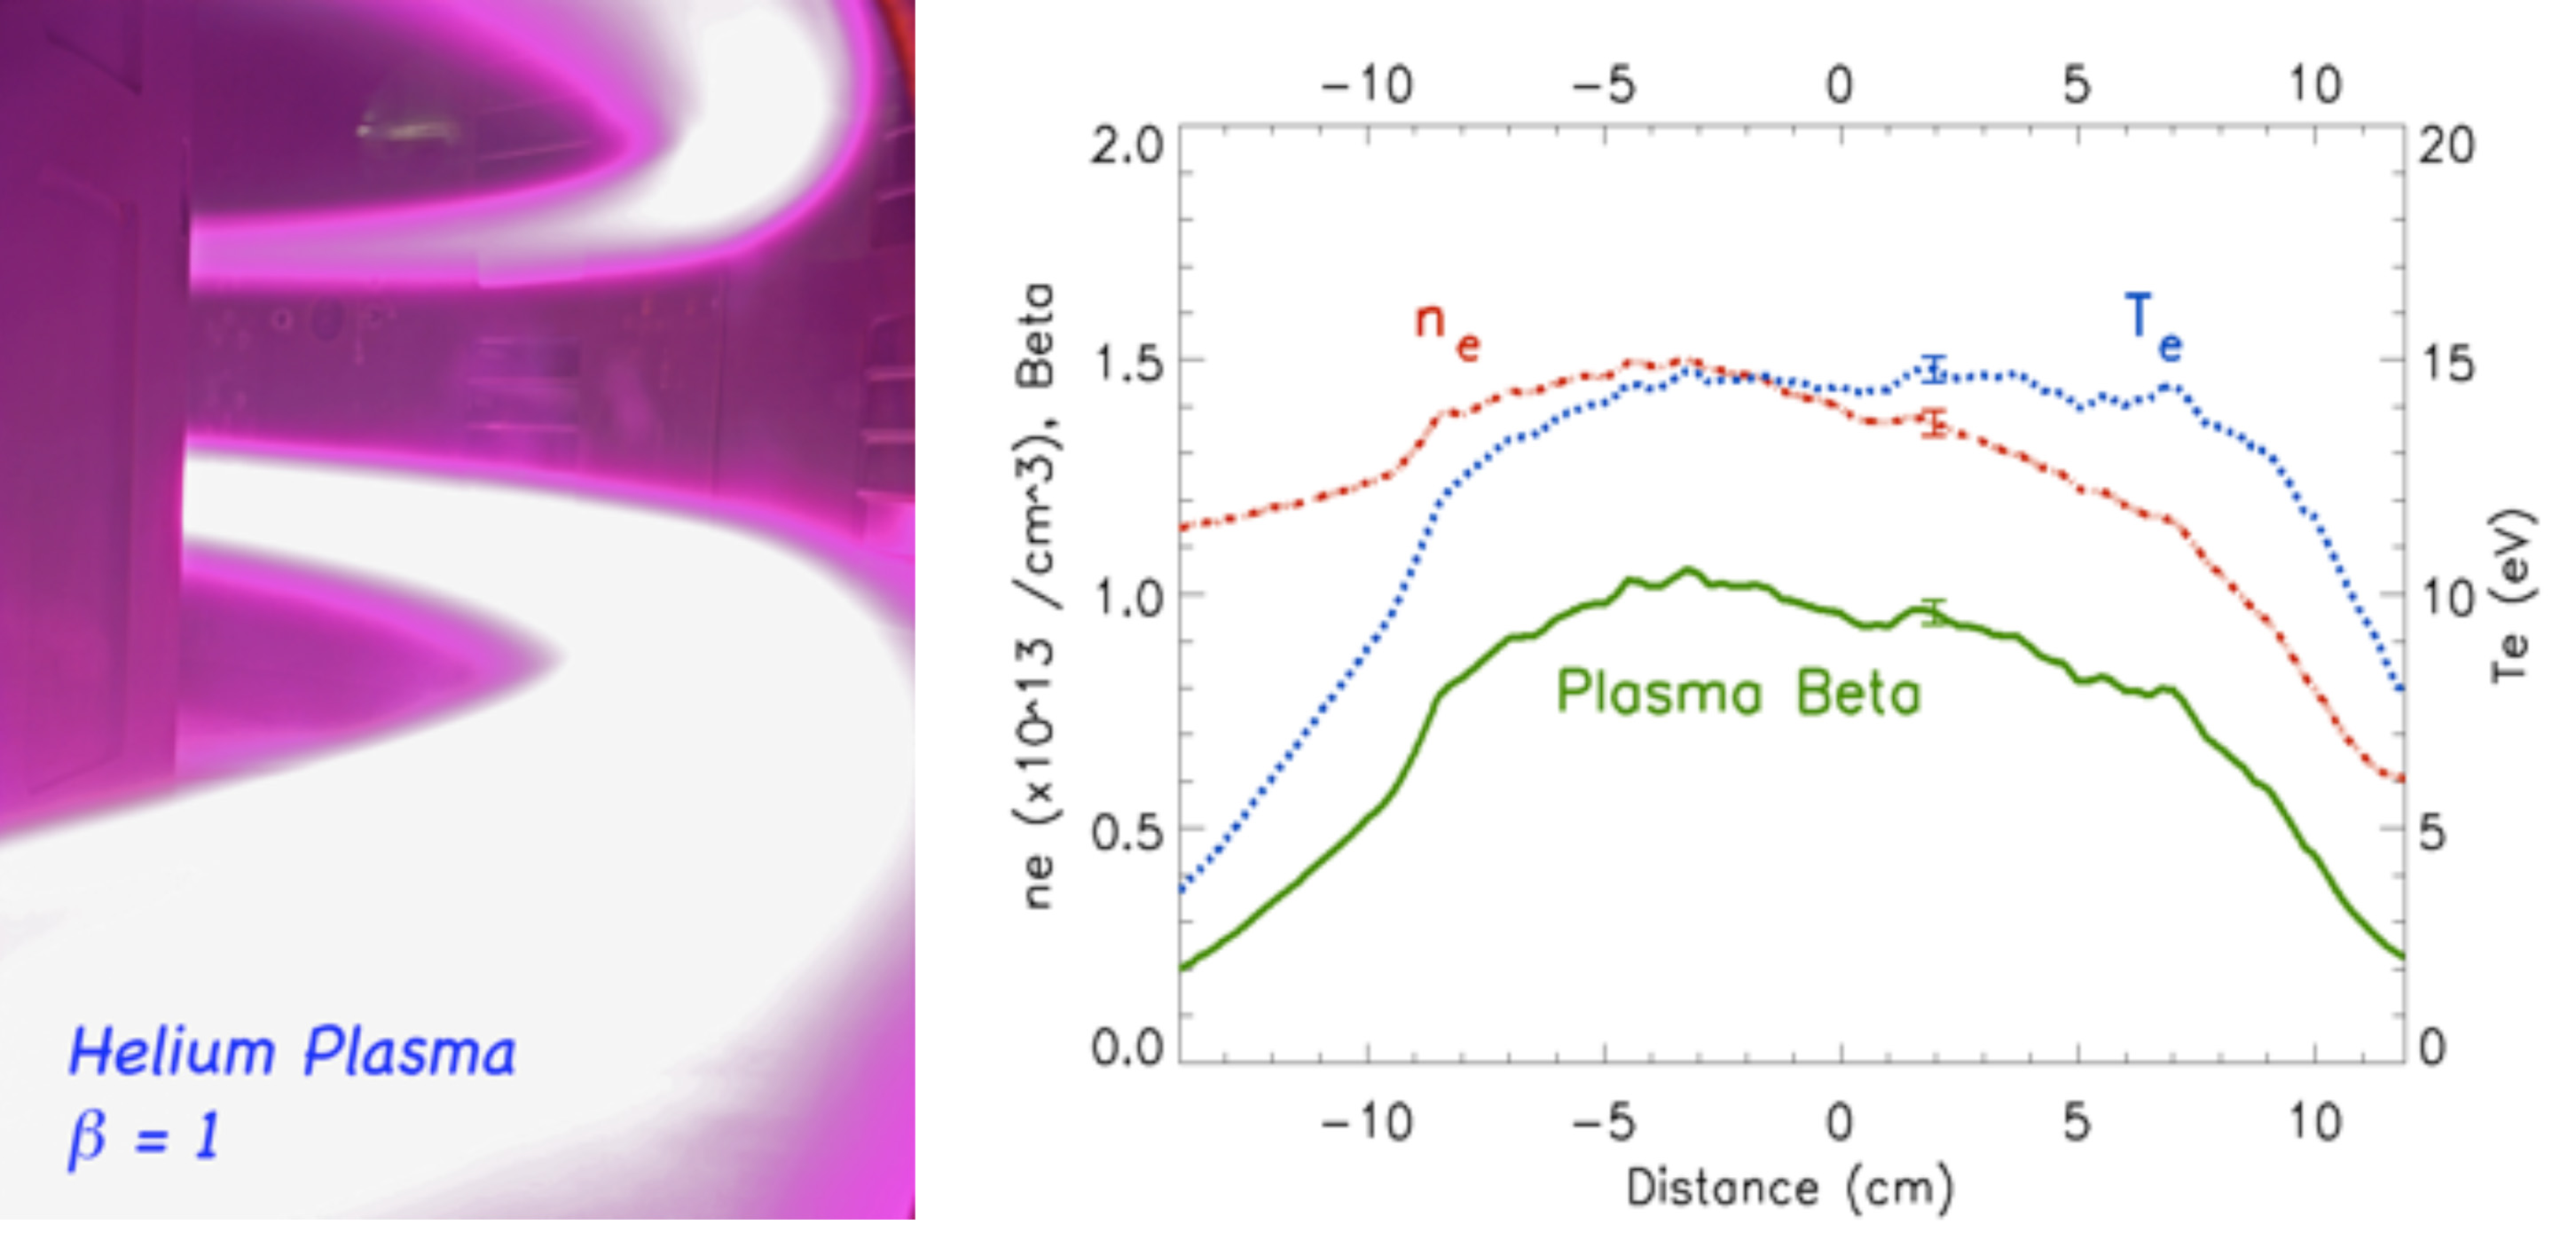
\includegraphics[width=0.9\textwidth]{etpd2.jpg} 
   \caption{ (left) Photograph of a helium plasma, using a vertical field to make the plasma spiral.  Each ring is 30 m in circumference.  The longest plasmas are 120 meters. (right) Plasma density and temperature measured with a Langmuir probe.  The ion temperature, measured spectroscopically, equals $T_{e}$. The central plasma beta is 1 at $B_{0}$ = 150G.  }
   \label{fig:etpd2}
\end{figure}

\pagebreak
\subsection{Low Temperature Plasma Device}


%\begin{wrapfigure}{l}{0.7\textwidth}
%  \centering
%   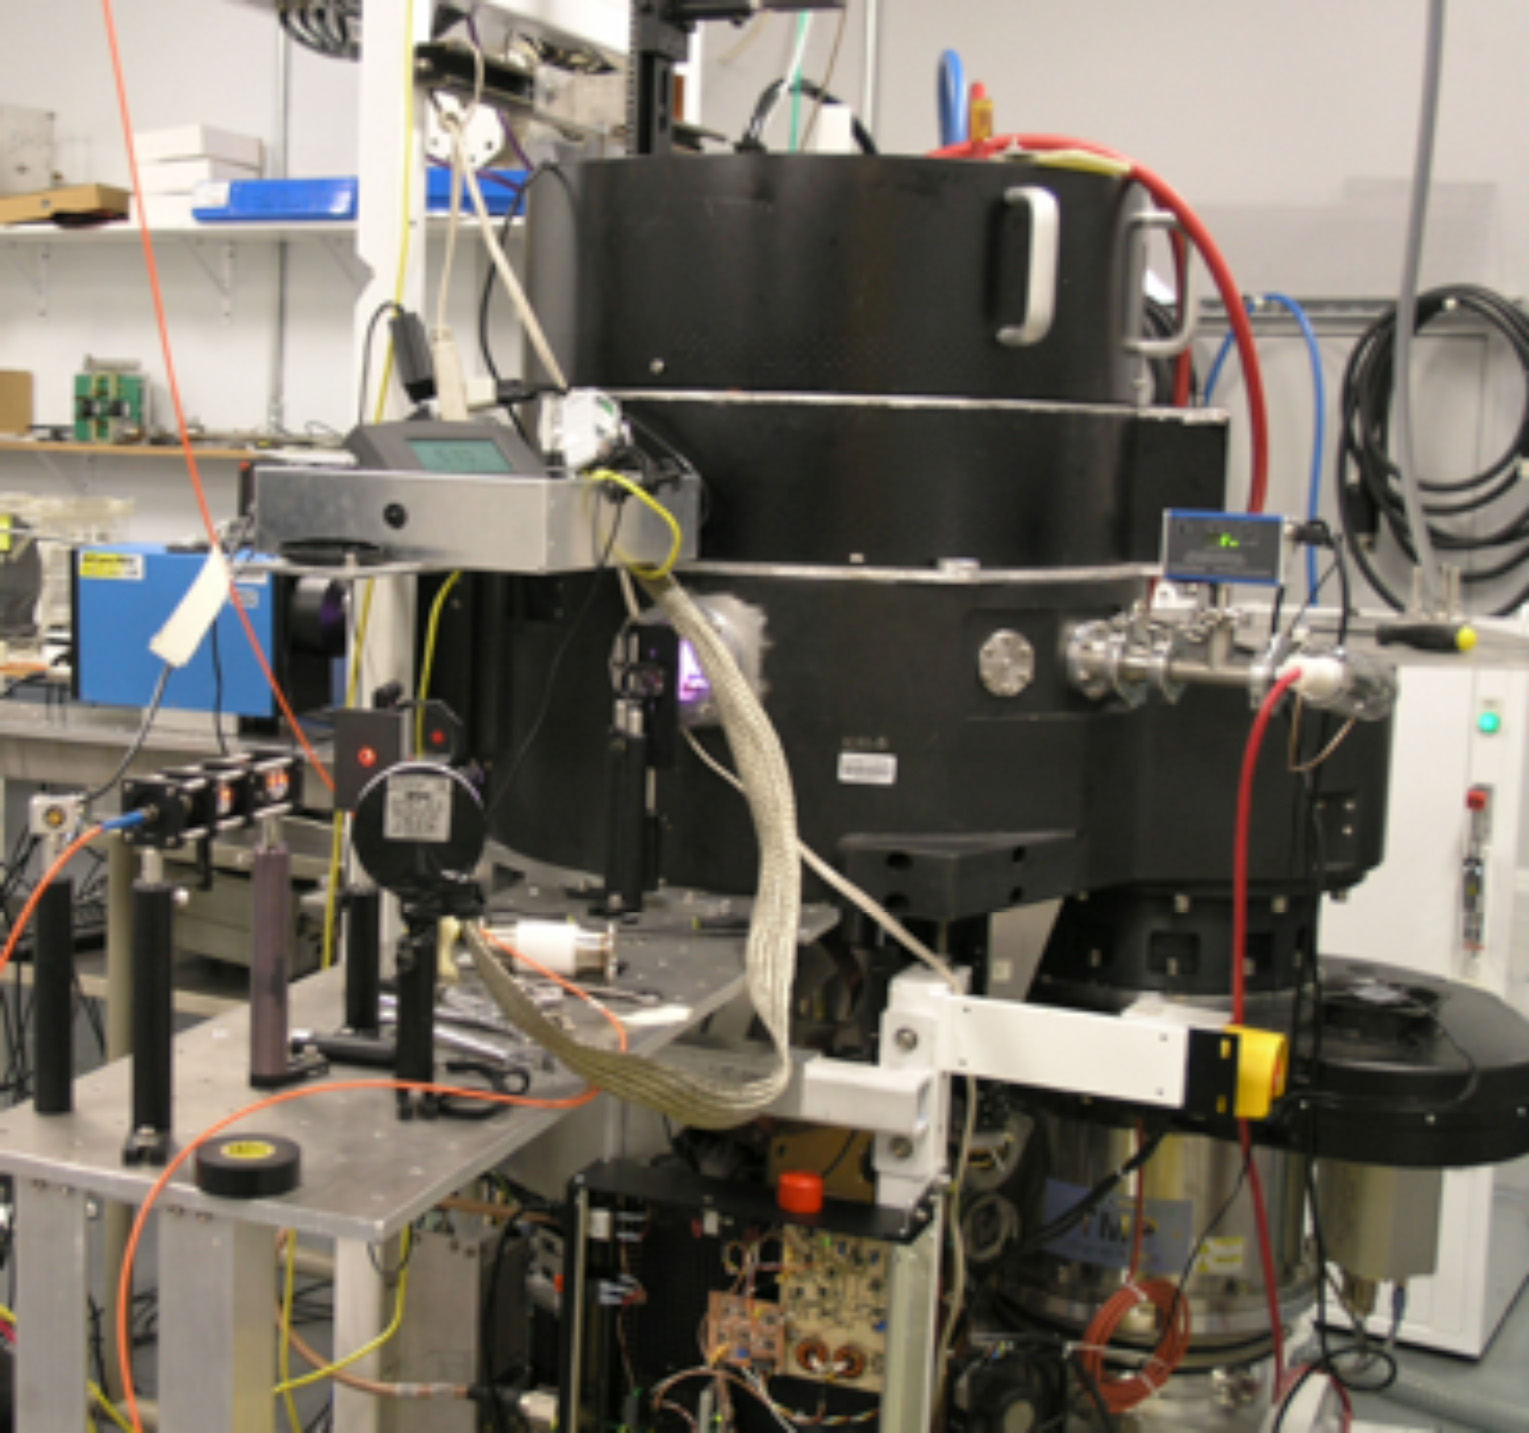
\includegraphics[width=0.65\textwidth]{etchtool.jpg} 
%   \caption{ \label{fig:etchtool}
%   Plasma etching tool donated by the Intevac Corp.  The tool was modified to allow LIF experiments and mount 2-D probe drives for wave studies.  The plasma is generated inductively and two separate frequencies are used for RF-bias (to accelerate ions to etch the wafer). The gases are fed by multiple mass-flow controllers and the machine is microprocessor controlled.}
%\end{wrapfigure}

A series of experiments on low temperature plasmas have been initiated at BaPSF with industrial partners.  The experiments have studied self-generated modes above a silicon wafer using correlation functions between emissive probes.  Laser Induced Fluorescence (LIF) has been used to measure the ion distribution as a function of height and phase during RF-biased acceleration in a plasma etching tool.  One such tool was donated by industry and is shown in Figure \ref{fig:etchtool}
\begin{figure}[h]
\centering
  \begin{minipage}[c]{0.5\textwidth}
    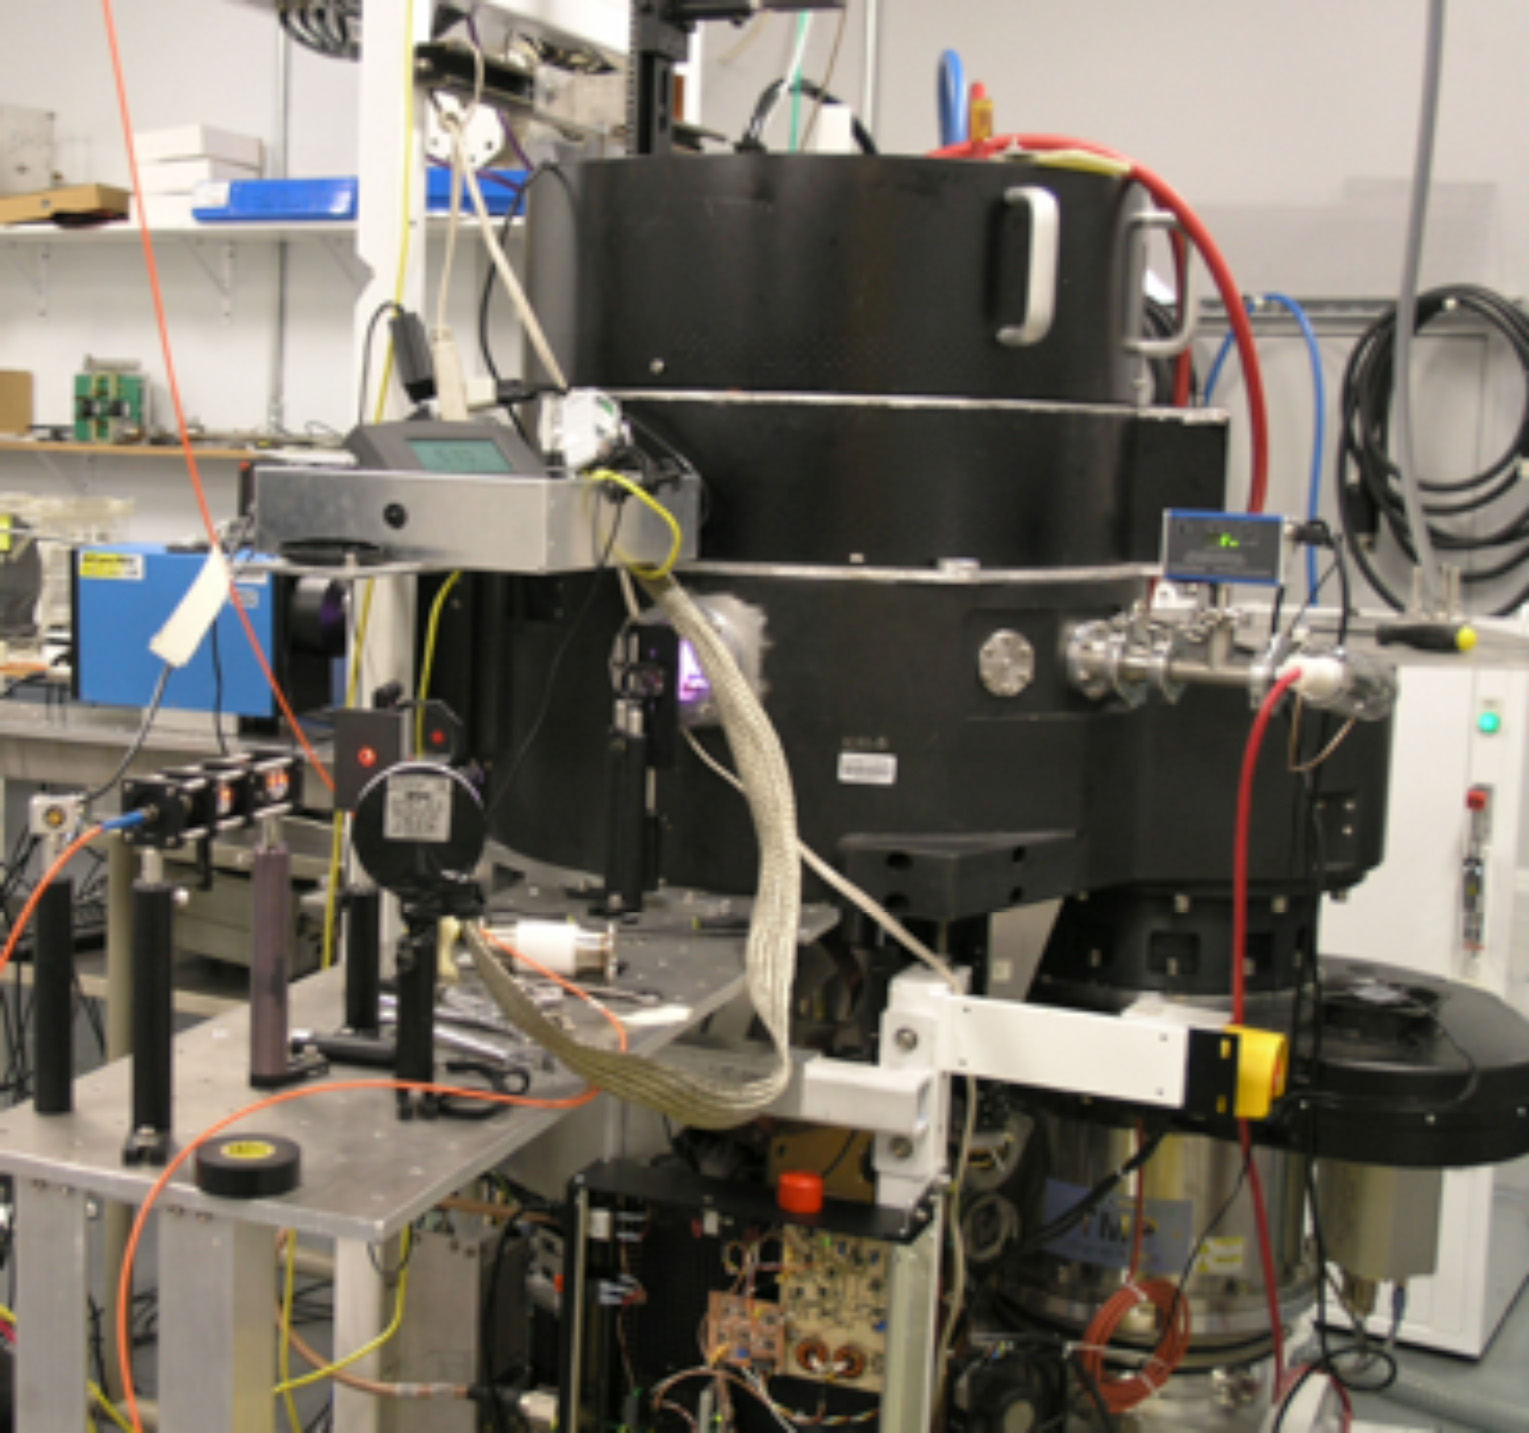
\includegraphics[width=\textwidth]{etchtool.jpg}
  \end{minipage}\hfill
  \begin{minipage}[c]{0.4\textwidth}
    \caption{Plasma etching tool donated by the Intevac Corp.  The tool was modified to allow LIF experiments and mount 2-D probe drives for wave studies.  The plasma is generated inductively and two separate frequencies are used for RF-bias (to accelerate ions to etch the wafer). The gases are fed by multiple mass-flow controllers and the machine is microprocessor controlled} 
    \label{fig:etchtool}
  \end{minipage}
\end{figure}

\subsection{4-meter Low Field Device}
A small test device, shown in Fig.\ \ref{fig:smpd}, was constructed using power supplies, a vacuum chamber and other hardware left over from the original 10 m-long LAPD device.  Magnetic field coils were wound from water-cooled welding cable that limits the background magnetic field to 300 G.  The plasma source is a 20 cm diameter LaB$_{6}$ cathode which makes plasmas of density   and the plasma is pulsed at 1 Hz.  The machine is an excellent device for testing probes, small beams and experimental techniques before using them in the LAPD device.  Users are welcome to utilize this machine for testing.  Presently it is also being used to conduct a solar flare experiment that involves installation of internal field coils that are not possible to move in and out of the LAPD.
\begin{figure}[htbp] %  figure placement: here, top, bottom, or page
   \centering
   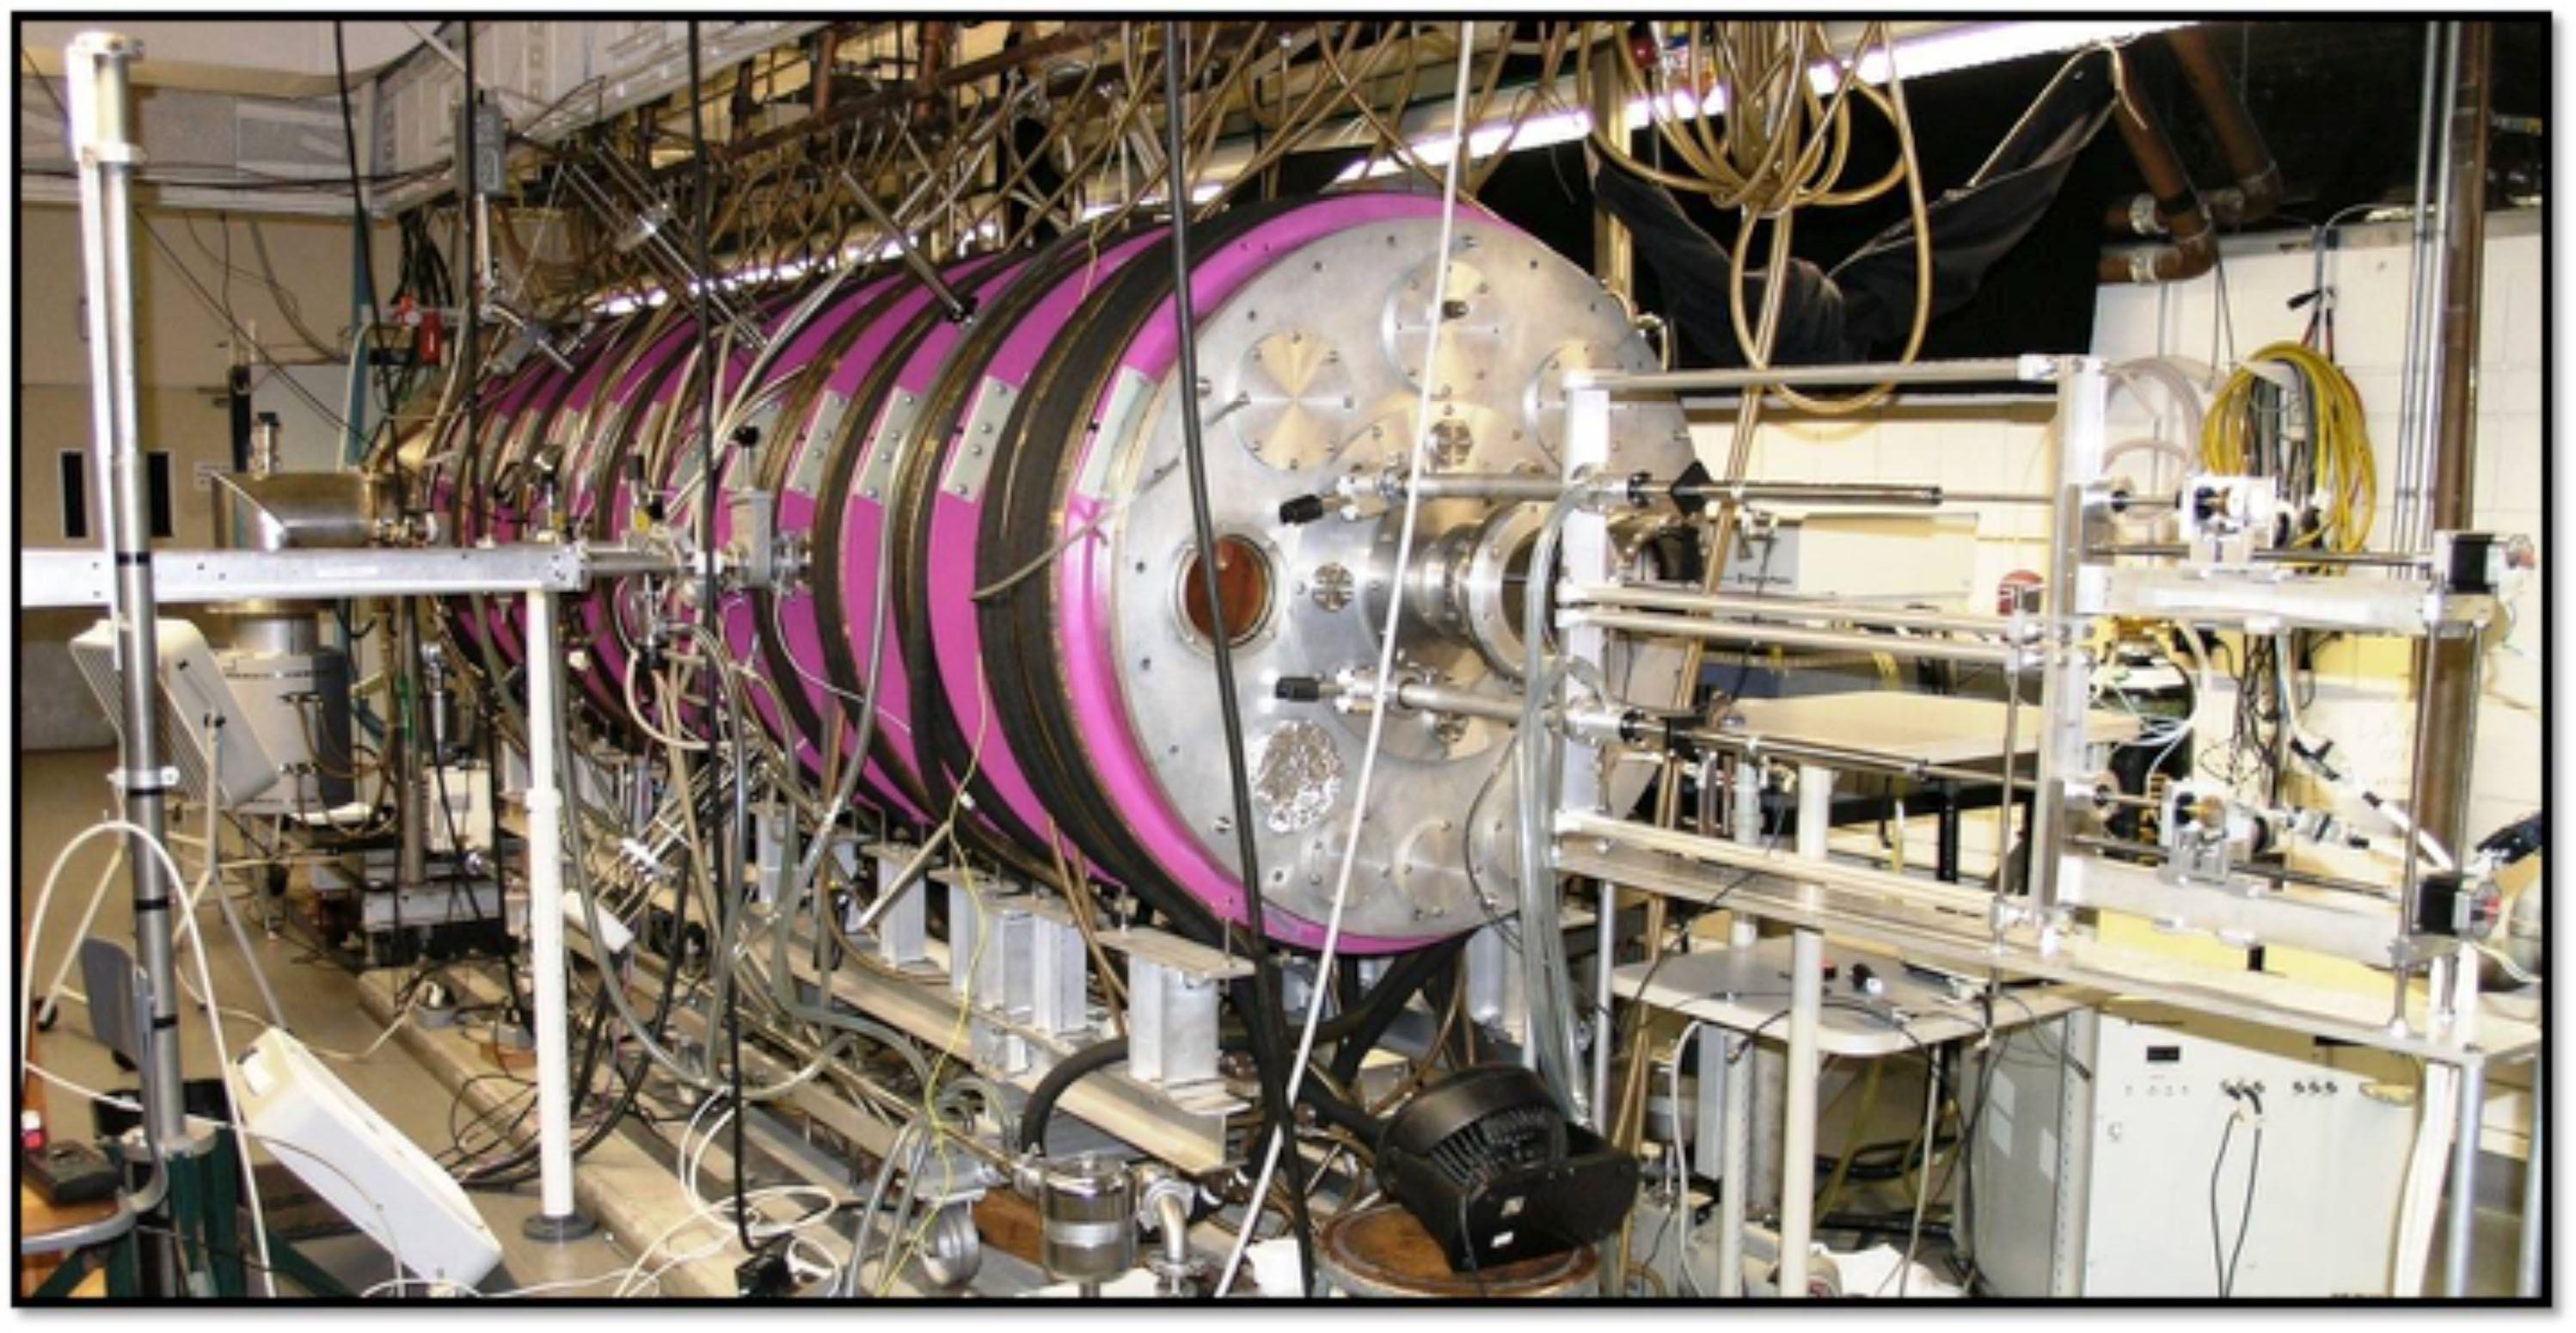
\includegraphics[width=0.85\textwidth]{smpd.jpg} 
   \caption{The SMPD, four-meter test chamber.  Probe drives for use in a solar flare experiment are on the right.}
   \label{fig:smpd}
\end{figure}



\subsection{LAPTAG High School Plasma Laboratory}
The BaPSF sponsors a high school outreach program known as the Los Angeles Physics Teachers Alliance Group  (LAPTAG).  High school students from the Los Angeles area use a small machine constructed especially for them out of spare parts and hand-me-down equipment from the facility.  The LAPTAG device is shown in Fig.\ \ref{fig:laptag}.  Any high school or community college student is welcome to participate in this program.  The students learn lab skills, build electronics and get lectures on plasma physics. The LAPTAG students have attended scientific meetings, including the APS-DPP annual meetings.  LAPTAG meets every Saturday and nearly every day during in the summer.
\begin{figure}[htbp] %  figure placement: here, top, bottom, or page
   \centering
   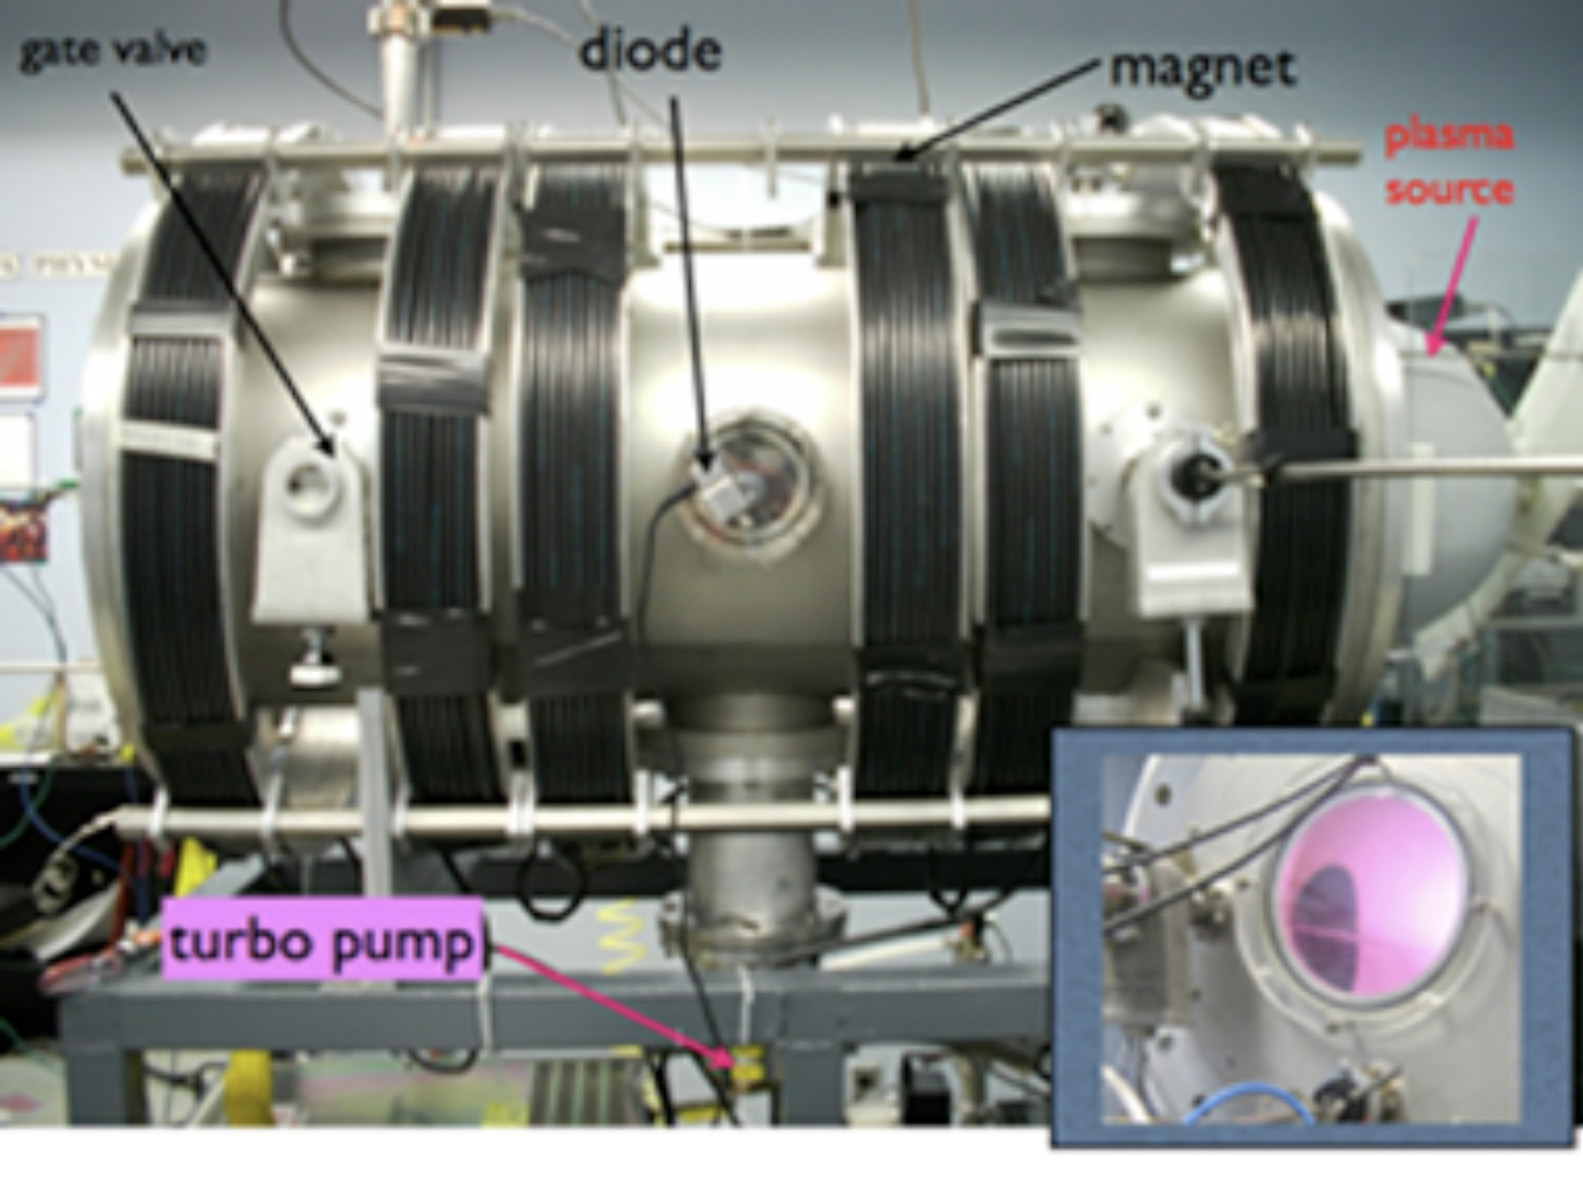
\includegraphics[width=0.75\textwidth]{laptag.jpg} 
   \caption{LAPTAG plasma physics device.  An inductively coupled plasma source makes a pulsed ($n_{e}\le 10^{11}$cm$^{-3}$) plasma with a background field of up to 100G.  The plasma is 2 m long and 40 cm in diameter}
   \label{fig:laptag}
\end{figure}


\subsection{Science and Technology Research Building (STRB)}
The LAPD and ETPD experiments and the low temperature physics laboratory are housed on two levels of the Science and Technology Research Building (STRB) on the West campus of UCLA.  The STRB is a relatively new (completed 1997) building which was designed to accommodate large experiments and/or those which require substantial electrical power.  There is 30 MW capability in the building.  A chilled water plant, recently upgraded, provides 55-degree (F) water to the STRB which is sufficient to cool 10 MW.  There is an additional chilled water system in the STRB. There is ample electrical power at 480, 220 and 120 Volts distributed throughout the building.  The ETPD area has several multi-megawatt transformers fed by 12 kV lines


\pagebreak
\subsection{Equipment Available to Users}

\subsubsection{Diagnostic Equipment}
Fifteen digital oscilloscopes, ranging from 2 channel-175 MHz/channel to one 4-channel 40 GHz scope (fpe < 12GHz in LAPD), 6 Stanford digital delay generators (1 ps accuracy), 2 BNC 8 channel pulse generators (1 ns accuracy), 1 LeCroy arbitrary waveform generator (10 MHz), 2 Agilent arbitrary waveform generators (80 MHz), HP 8568B spectrum analyzer, Agilent Network Analyzer (to 180 MHz), 12 channels of Tektronix-Sony 100 MHz optical isolators, 2 microscopes for probe construction (one with micro-manipulators.)\\
	A range of digitizers are available for facility users, including
\begin{itemize}
\item Thirty-two channels of 100MHz/chan, 1MS/chan at 16-bit vertical resolution.
\item Sixty-four  channels of 100 MHz/chan, 128kS/chan, 14-bit digitizers.
\item Sixteen channels at 1.25GHz/chan, 256GS/chan, 10 bit resolution-- optionally scalable to four channels at 5GHz/chan.

\item The 40GHz oscilloscope can be used as an 8-bit digitizer and is integrated into the data acquisition system.
\end{itemize}
	An array of 7, 56GHz microwave interferometers operates in LAPD at 1Hz providing diagnostic density measurements at 7 fixed axial locations along the plasma column. One portable, 96GHz interferometer is available for high-density $ \sim 10^{13}$ measurements.

\subsubsection{Amplifiers, Sources for Launching Waves}
One custom-built 30 kW amplifier (may be tuned for 200 kHz-5 MHz operation), 1 Velonix 360 high voltage pulser (up to 30 kV pulses, 100 ns rise-time), 1 AR 2500L, 10 kHz-220 MHz, 2.5 kW broadband amplifier, 1 AR 2000L, 10 kHz-220 MHz, 2 kW broadband amplifier, 1 AR 200L 1 MHz-200 MHz, 200 W broadband amplifier, 1-250 kW (2.5 ms pulse) 9 GHz source.

\subsubsection{Lasers}
Two Nd:YAG pumped lasers with 7 ns, 150 MW pulse (up to 10 Hz); one with a frequency doubling (532-nm) crystal.  One CW tunable dye laser: bandwidth 1 MHz, free spectral range 30 GHz, power up to 1-Watt (Coherent 899 driven by an INNOVA Argon ion laser) mounted on an air-isolated optical bench (Spectra Physics Pro 290).  Optics are on hand to operate in the blue to far red depending upon choice of dye. Equipment associated with this laser is: a confocal spectrum analyzer, New-Focus 7711 Fizeau Wavelength meter, iodine cell, opto-acoustic light chopper and light detection phototubes, amplifiers and power supplies.  The newest addition is a pulsed dye laser (10 ns pulse and 100 ns pulse stretcher) 2-12 MW programmable, spectral output from 270-700 nm for LIF photography.  This is coupled with a Cooke Gen III, high speed (tmin = 3 ns), (1024X1280 pixel CCD), computer controlled camera with averaging and background subtraction capabilities.  This camera is for the imaging of planar LIF signals. Both lasers are interfaced to computers and can be driven by the data acquisition system or used independently.

\subsubsection{Energetic Ion Beam}
An ion beam source has been developed at BaPSF to perform experiments related to the Fast-Ion Campaign.  The beam source was constructed by Drs. S. Tripathi and P. Pribyl, and Prof. W. Gekelman.  It delivers an 18 kV, 3 Amp, He-ion beam.  The energy is chosen to match the phase velocity of Alfv\'{e}n waves in the LAPD.  Figure 9F is a photograph of the beam source attached to the LAPD device.  The beam source consists of a plasma generator, which is based on a pulsed, inductively-coupled antenna.  A pulsed 25 kV power supply was designed and constructed to accelerate the beam.  This design has the safety feature that high-voltage on the grids is present for only a few milliseconds. 
 The beam uses three focusing grids (obtained from an old neutral beam source used at PPPL) and enters into a drift chamber where several turbo pumps and Carbon baffles remove neutrals that drift-in from the plasma-source region.  This configuration is also necessary to prevent excessive beam loss due to charge exchange collisions.
	Recently, the performance of the ion beam source has been greatly improved by replacing the copper grids with grids made of molybdenum, and by optimizing the grid spacing.  Figure 10A shows the radial profile of the measured beam-current density 4.28 meters from the beam injection point in the LAPD.  The maximum beam density is $n_{b} = 10^{8}$ cm$^{-3}$. A second large  improvement occurred when the RF source at the end of the chamber was replaced with a LaB$_{6}$ cathode based source.

The effect of the injected beam on the ambient LAPD plasma has been documented; a wave generated, probably by Cherenkov radiation, is observed. Figure 11A shows a snapshot of the fluctuating vector magnetic field triggered by the beam injection.  The ion beam has been an important tool for the Fast-Ion Campaign lead by Prof.W. Heidbrink, but it is also available to all BaPSF users who request it for their projects.   More recently, it was used by the Los Alamos group headed by Pat Colestock to test code predictions.
\begin{figure}[htbp] %  figure placement: here, top, bottom, or page
   \centering
   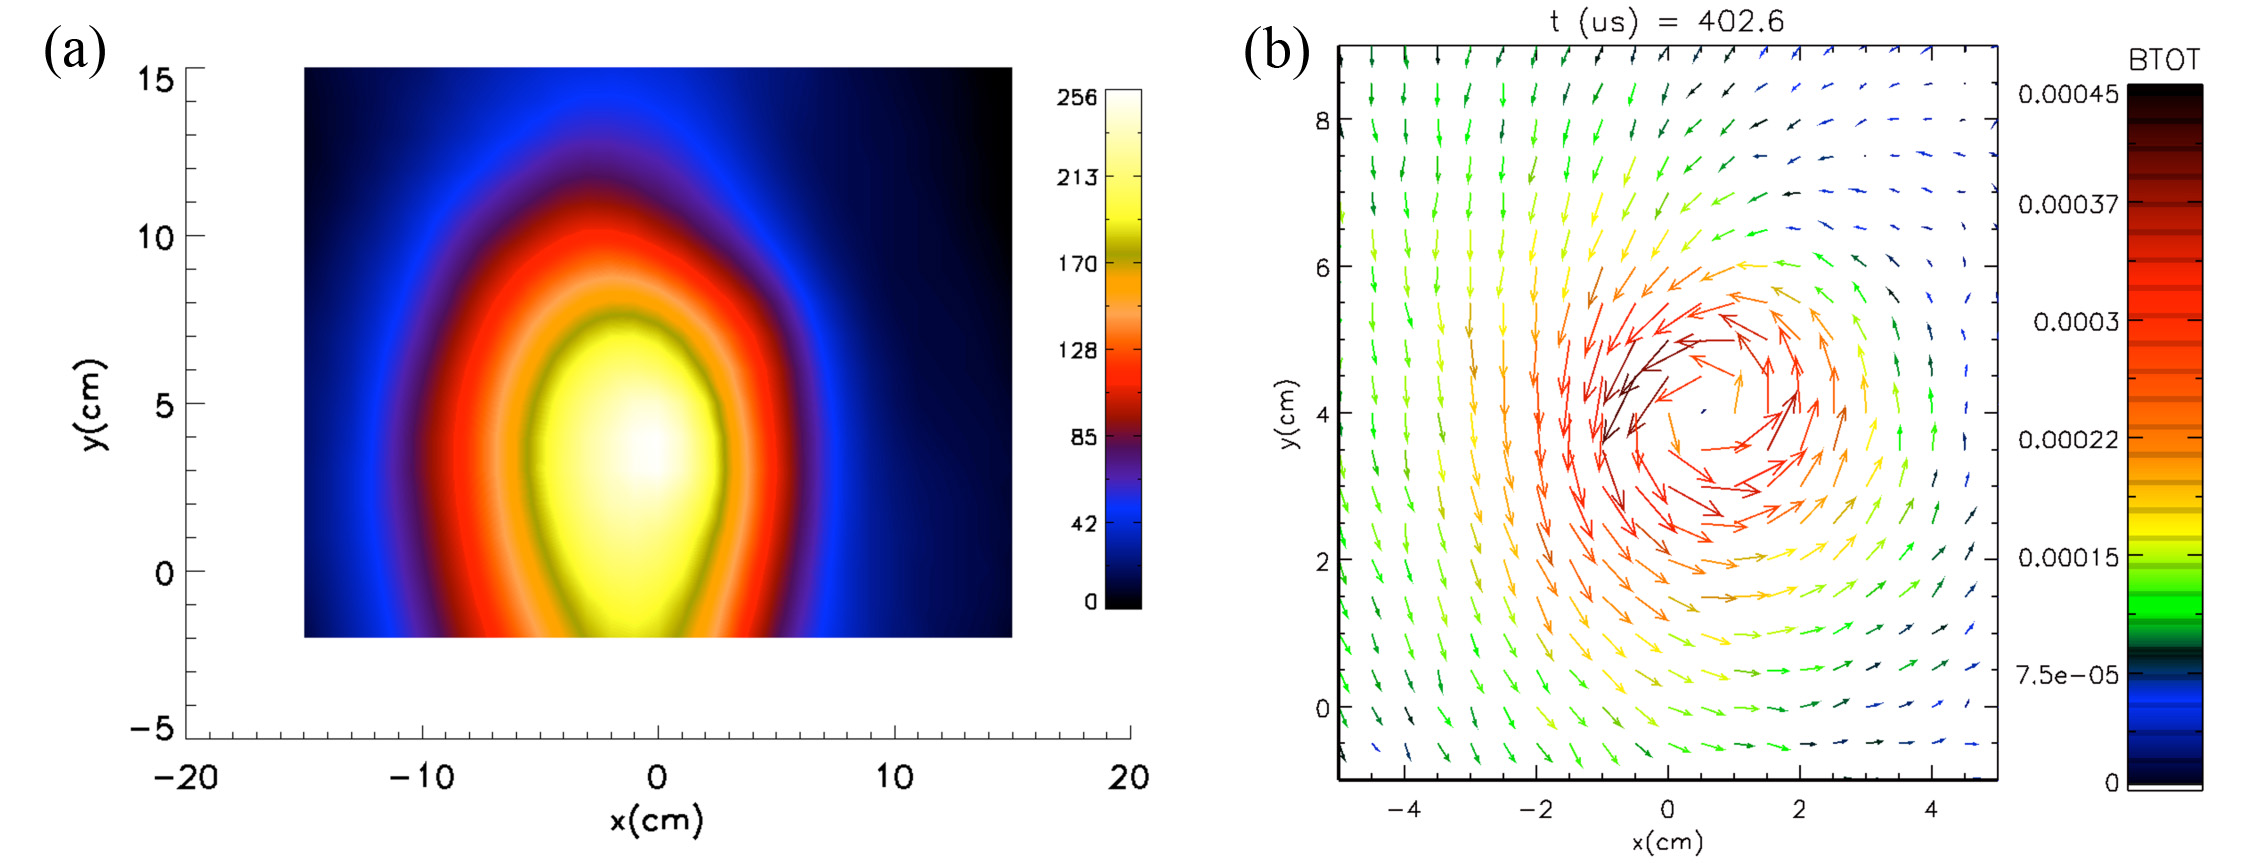
\includegraphics[width=0.95\textwidth]{ionbeam_and_wave.jpg} 
   \caption{(a) Helium ion beam ($V_{beam}$ = 22 keV) profile 4.28 m away from the beam source.  The brightest region corresponds to $n_{b} = 10^{8} $cm$^{-3}$. (b) Vector map of the fluctuating magnetic field excited by the ion beam .  Mode frequency is 510 kHz, ion cyclotron frequency 513 kHz.  $V_{beam} = 22$ keV, $I_{beam} = 0.42$ A, LAPD magnetic field is 1.35 kG, background plasma density $n = 1.8 \times 10^{12}$ cm$^{-3}$. }
   \label{fig:ionbeam_and_wave}
\end{figure}
 
 \subsection{Communications and Computing}
The computer network at the BaPSF comprises its own public class-C network for general computing and several internal private subnets for data acquisition and machine control. Gigabit network switches are available throughout the facility. In 2009 UCLA invested \$80k (at no cost to the facility) to replace the three main, but aging, Cisco switches in the STRB with state-of-the-art versions, having 10 GBit uplinks to the UCLA campus backbone. Wireless (B/G/N) network connectivity is also provided to the users in both the STRB and offices. 
	Data storage resources at BaPSF include a 48TB RAID 6, centralized network storage server, with a second server providing daily, incremental disk-to-disk backups; a tape backup system is also used for data archiving. Facility users have access to several Linux workstations as well as a main computer server with 64GB RAM and 8 Intel Xeon processor cores. In addition, the facility and local resources include 6 Windows systems (for experiment data acquisition, automated probe motion, machine state monitoring, diagnostics, and control) and 7 Mac computers; one Mac is configured for advanced data visualization using Maya software with custom data import and analysis plug-ins. Output from this visualization computer can be viewed on a 72-inch, 3D HDTV using LED shutter glasses. Workstations have IDL and Maya for scientific visualization as well as several language compilers (C, C++, and Fortran). Two color laser printers, a slide scanner, and a flatbed scanner are also available.  The facility website is hosted by a dedicated departmental server, and may be accessed at this URL: http://plasma.physics.ucla.edu/bapsf

%\newpage

%\setcounter{page}{1}

%\bibliographystyle{unsrtnat}
%\bibliographystyle{prsty}
%\bibliographystyle{unsrt}
%\bibliography{refs}  




\end{document}
